\documentclass[conference]{IEEEtran}

\usepackage{amsmath}
\usepackage{amsfonts}
\usepackage{graphicx}
\usepackage{cite}
\usepackage{float}
\usepackage{hyperref}
\hypersetup{
    colorlinks=true,
    linkcolor=blue,
    citecolor=blue,
    filecolor=blue,
    urlcolor=blue,
}

\begin{document}

\title{Control Design and MATLAB Simulation of a Ball-and-Beam System Using Pole Placement}

\author{
    \IEEEauthorblockN{Alexander J. Brown}
    \IEEEauthorblockA{Department of Electrical Engineering\\
    University of Alabama in Huntsville\\
    Email: ajb0083@uah.edu}
}

\maketitle

\begin{abstract}
    This paper presents the modeling and control of a ball-and-beam system, a classic example of instability in control theory. The system dynamics were derived using Newtonian and Lagrangian mechanics, providing a robust foundation for control design. Two state-feedback controllers were implemented: Pole Placement using Ackermann’s formula and a Linear Quadratic Regulator (LQR). Simulation results demonstrated both controllers' ability to stabilize the system, with the LQR controller achieving superior performance in terms of energy efficiency and transient response. Key metrics, including Integral of Absolute Error (IAE), Integral of Squared Error (ISE), and Integral of Time-weighted Absolute Error (ITAE), showed a 3.56\% improvement in smoothness and stability for the LQR controller compared to Pole Placement. These findings were validated using MATLAB simulations and real-time 3D visualizations, highlighting the practical viability of the proposed control strategies. This study provides valuable insights into trade-offs between control robustness and rapid stabilization for inherently unstable systems.
\end{abstract}

\begin{IEEEkeywords}
    Ball-and-Beam system, Lagrangian mechanics, Newtonian mechanics, State-space representation, Control design, LQR controller, Pole Placement, MATLAB simulation, feedback control, modern control systems.
\end{IEEEkeywords}
    

\section{Introduction}
\label{sec:intro}
The ball-and-beam system is a fundamental example in control theory, widely recognized for its simplicity in structure yet inherent instability. The system consists of a ball rolling along a beam, manipulated by a control mechanism to maintain its position. Its instability and coupled dynamics make it an ideal model for teaching and developing control strategies, emphasizing system modeling, stability analysis, and feedback design.

\subsection{Background of the Problem and Importance}
\label{subsec:intro_background}
The ball-and-beam system has been extensively used in academia and industry to demonstrate key principles of control engineering. Beyond its instructional value, its dynamics are representative of real-world applications, such as balancing robots, flight control systems, and load stabilization in cranes. These applications share common challenges, including nonlinearity, instability, and the need for rapid, precise control. The ability to stabilize such systems through advanced control techniques highlights the relevance of the problem.

\subsection{Literature Review and Motivation}
\label{subsec:intro_lit_review}
The modeling and control of ball-and-beam systems have been the subject of numerous studies. Bolívar and Beauchamp \cite{bolivar2014} demonstrated the utility of combining Newtonian and Lagrangian mechanics to achieve accurate modeling of system dynamics. Norlander \cite{norlaner2003} introduced flexible frameworks for pole placement, enabling control designers to fine-tune system responses. Umar et al. \cite{umar2022} highlighted the LQR controller's efficiency in balancing performance and energy usage in a Ball-on-Sphere system.

While these studies underscore the effectiveness of state feedback methods, there remains a gap in directly comparing these strategies—Pole Placement and LQR—under identical conditions for the ball-and-beam system. This study builds upon the insights provided by prior research by implementing and rigorously evaluating these control strategies.

\subsection{Overview of the Problem and Approach}
\label{subsec:intro_overview}
This study focuses on developing and comparing two state feedback controllers—Pole Placement via Ackermann’s formula and Linear Quadratic Regulator (LQR)—for the ball-and-beam system. Using a state-space representation derived from Newtonian and Lagrangian mechanics, the controllers are designed to stabilize the system and improve performance. Validation is achieved through MATLAB simulations, Simulink models, and real-time 3D visualizations.

The key contribution of this paper lies in its direct comparison of these control strategies, emphasizing the trade-offs between rapid stabilization and smooth control effort. By implementing these controllers and assessing their performance through metrics such as stability, transient response, and energy efficiency, this study provides actionable insights for control system design.

\section{Background and Problem Formulation}
\label{sec:background}
The ball-and-beam system represents a classic challenge in control engineering due to its inherent instability. It consists of a beam, pivoted at its center, and a ball that rolls along its surface. The objective is to control the beam's angle to stabilize the ball at a desired position. This problem captures the essence of instability, where even minor disturbances can cause significant deviations in the system.

\subsection{General Background and Importance}
\label{subsec:general_background}
In real-world applications, systems like the ball-and-beam exhibit similar dynamics, such as balancing robots and aircraft flight controls. These systems often operate near critical points of instability and require robust control strategies to maintain balance. Solving the ball-and-beam problem is not only academically valuable but also critical for advancing practical control systems capable of handling similar challenges.

\subsection{Problem Definition and Challenges}
\label{subsec:problem_definition}
The primary challenge in the ball-and-beam system is its nonlinear and coupled dynamics. The position of the ball is influenced by the beam's angle, which, in turn, is controlled externally. This coupling makes the system highly sensitive to disturbances, necessitating precise modeling and robust control strategies.

This study addresses these challenges by deriving a state-space representation of the system from first principles, enabling the implementation of modern control techniques. The problem is further complicated by the need to balance transient response and steady-state performance while minimizing energy consumption. These considerations define the scope and objectives of this work.

\section{Methodology: System Modeling and Controller Design}
\label{sec:methodology}

This section details the mathematical modeling of the ball-and-beam system and the design of feedback controllers for stabilization. The methodologies applied include deriving the system dynamics using Newtonian and Lagrangian mechanics and developing controllers using state-space representation.

\subsection{System Modeling Using Newtonian and Lagrangian Mechanics}
\label{subsec:modeling}
Accurate modeling of the ball-and-beam system is critical for understanding its dynamic behavior and designing an effective control strategy. This section presents two approaches to deriving the system dynamics: Newtonian mechanics, based on principles of force and torque, and Lagrangian mechanics, which utilizes energy-based analysis.

\begin{figure}[H]
    \centering
    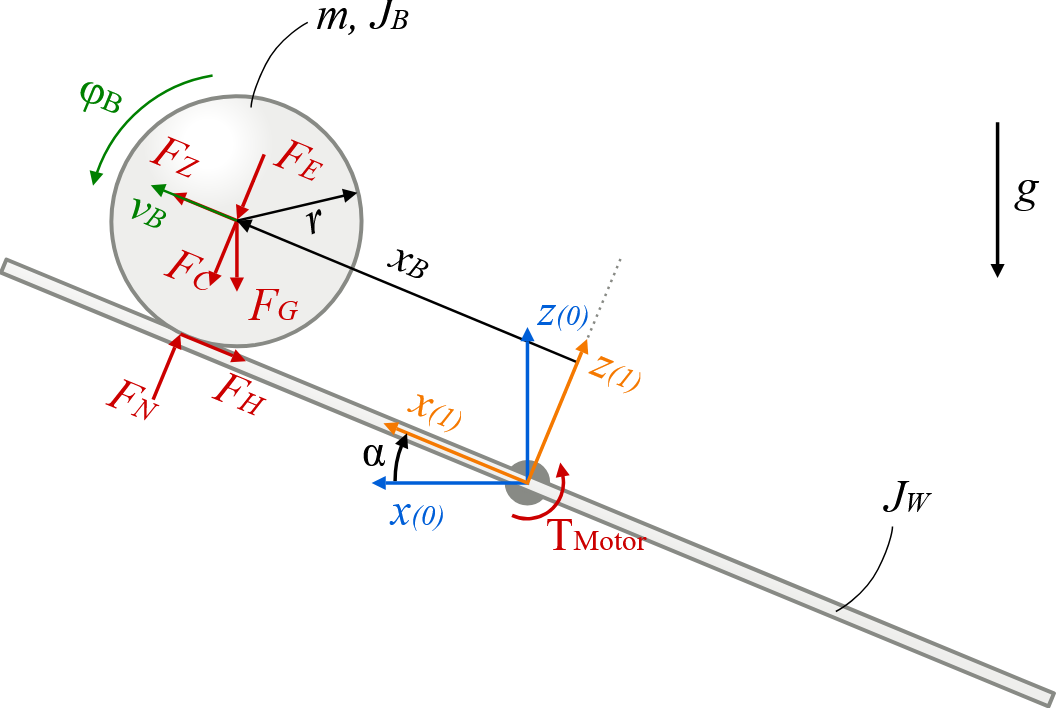
\includegraphics[width=0.8\linewidth]{Figures/system_diag_wiki_right.PNG}
    \caption{Schematic of the Ball-and-Beam System. The figure shows the key parameters, including ball displacement \(x_B\), beam angle \(\alpha\), and forces acting on the system. Adapted from \cite{mager2015}.}
    \label{fig:ball_beam_schematic}
\end{figure}

\subsubsection{Newtonian Mechanics}
\label{subsubsec:model_newtonian}
Using Newton's second law for translational and rotational dynamics, the coupled motions of the ball and beam are derived. The equations for the ball's motion and beam's rotation are:
\begin{equation}
\ddot{x} = -g \sin(\theta), \quad \ddot{\theta} = -\frac{m g x \cos(\theta)}{I},
\end{equation}
where \(x\) is the ball's position, \(\theta\) is the beam's angle, \(g\) is gravitational acceleration, \(m\) is the ball's mass, and \(I\) is the beam's moment of inertia.

\subsubsection{Lagrangian Mechanics}
\label{subsubsec:model_lagrangian}
Lagrangian mechanics offers a systematic approach by defining the Lagrangian as:
\begin{equation}
\mathcal{L} = T - V = \frac{1}{2}m\dot{x}^2 + \frac{1}{2}I\dot{\theta}^2 - m g x \sin(\theta),
\end{equation}
where \(T\) and \(V\) are the kinetic and potential energies, respectively. Using the Euler-Lagrange equation, the equations of motion are derived:
\begin{equation}
m\ddot{x} = -m g \sin(\theta), \quad I\ddot{\theta} = -m g x \cos(\theta).
\end{equation}

\subsubsection{State-Space Representation}
\label{subsubsec:model_ss}
The system is linearized around its equilibrium point (\(x = 0, \theta = 0\)) and represented in state-space form:
\begin{equation}
\dot{\mathbf{x}} = A\mathbf{x} + B u, \quad \mathbf{y} = C\mathbf{x} + D u,
\end{equation}
where \(\mathbf{x}\) is the state vector, \(u\) is the control input, and matrices \(A, B, C, D\) encapsulate the system dynamics.

\subsection{Controller Design}
\label{subsec:controller_design}
Two state feedback control strategies—Linear Quadratic Regulator (LQR) and Pole Placement—were implemented to stabilize the ball-and-beam system. These strategies were chosen for their theoretical grounding in modern control theory and their complementary approaches to stabilizing linearized systems.

\subsubsection{Linear Quadratic Regulator (LQR)}
\label{subsubsec:lqr}
The LQR controller is a widely used optimal control method that minimizes a quadratic cost function:
\begin{equation}
J = \int_{0}^{\infty} (\mathbf{x}^\top Q \mathbf{x} + u^\top R u) dt,
\end{equation}
where \(Q\) and \(R\) are symmetric positive semi-definite and positive definite weighting matrices, respectively. These matrices define the trade-offs between state deviations and control effort. For this study, the matrices were selected as:
\[
Q = \text{diag}(200, 10, 10, 10), \quad R = 1,
\]
to emphasize precision in the ball's position while penalizing excessive control effort. The feedback gain matrix \(K_{\text{lqr}}\) was computed using MATLAB's built-in \texttt{lqr} function, which solves the associated algebraic Riccati equation.

The LQR controller was implemented to achieve smooth transient responses with minimal overshoot and oscillations. The optimal design ensures a balance between settling time and control effort, making it particularly suitable for applications requiring energy efficiency and steady-state precision. The robustness of this approach under parameter variations, such as changes in mass and beam length, was validated through sensitivity analysis, as described in Section~\ref{subsec:sensitivity_analysis}.

\subsubsection{Pole Placement}
\label{subsubsec:pole_placement}
The Pole Placement method, implemented using Ackermann’s formula, is a deterministic control strategy that directly places the closed-loop poles at desired locations. For this study, the poles were selected as:
\[
[-158, -2+3i, -2-3i, -3.5],
\]
to mimic the dynamic behavior of the LQR controller while achieving rapid stabilization. The feedback gain \(K_{\text{acker}}\) was computed using MATLAB’s \texttt{acker} function.

Pole Placement provides explicit control over the system’s dynamics by allowing designers to specify desired eigenvalues of the closed-loop system. However, the choice of pole locations significantly influences the system's transient response and sensitivity to parameter variations. While this method ensures rapid stabilization, it was observed to produce higher control effort and transient oscillations under certain parameter changes. These characteristics highlight the trade-off between response speed and control robustness.

\subsubsection{Backsolving Approach for Direct Comparison}
\label{subsubsec:backsolving}
A key challenge in this study was selecting pole locations which effectively stabilized the system without excessive oscillations or control effort. This was addressed using an innovative backsolving approach suggested by Jonathan Shreve and Garret Smith, as detailed in the Acknowledgment section of this report. The backsolving method facilitated the alignment of pole placement objectives with the dynamics achieved by the LQR controller, enabling the specification of pole locations that closely mirrored the LQR's performance metrics.

This approach ensured that the Pole Placement controller's dynamic performance was comparable to that of the LQR controller, providing a consistent baseline for evaluating their respective strengths and weaknesses. By leveraging the backsolving technique, it was possible to directly assess the trade-offs in terms of transient response, control effort, and sensitivity to parameter variations, as detailed in Section~\ref{sec:experiment_analysis}.

\section{Experimentation and Simulation Analysis}
\label{sec:experiment_analysis}

This section describes the experimental setup, parameter tuning, and results of the LQR and Pole Placement controllers. Simulations were performed using MATLAB and Simulink, starting with an initial state vector:
\[
\mathbf{x}_0 = \begin{bmatrix} -0.2 \\ 0 \\ 0 \\ 0 \end{bmatrix},
\]
representing an initial displacement of \(-0.2\) meters. Both controllers shared identical system parameters for a fair comparison.

The LQR controller was tuned using weighting matrices to prioritize smooth transitions and stability, while the Pole Placement controller's desired pole locations were derived from the LQR controller's closed-loop dynamics.

Performance metrics such as Integral of Absolute Error (IAE), Integral of Squared Error (ISE), and Integral of Time-weighted Absolute Error (ITAE) were used to evaluate the controllers. Table~\ref{tab:performance_metrics} summarizes the results:

\begin{table}[H]
\centering
\caption{Performance Metrics for Pole Placement and LQR Controllers}
\label{tab:performance_metrics}
\begin{tabular}{|c|c|c|c|}
\hline
\textbf{Controller} & \textbf{IAE}   & \textbf{ISE}   & \textbf{ITAE}  \\ \hline
Pole Placement      & 0.13262        & 0.01937        & 0.05834        \\ \hline
LQR                 & 0.13314        & 0.01975        & 0.05626        \\ \hline
\end{tabular}
\end{table}

The LQR controller excelled in minimizing late-stage errors (ITAE), making it suitable for applications requiring smooth convergence. The Pole Placement controller demonstrated better error tracking over time (IAE) due to its aggressive stabilization approach.

MATLAB simulations suggests that the LQR controller achieves smoother transitions with minimal overshoot, while the Pole Placement controller stabilizes more rapidly but introduces transient oscillations. Figure~\ref{fig:state_sim} illustrates the state responses and control inputs.

\begin{figure}[H]
    \centering
    \includegraphics[width=0.8\linewidth]{Figures/matlab_simulation.PNG}
    \caption{State variable responses (\(x, \theta\)) and Control Input effort (\(u\)) for both control schemes in MATLAB Simulation.}
    \label{fig:state_sim}
\end{figure}

Both controllers effectively stabilized the ball-and-beam system. The LQR controller showed slighly more precision and energy efficiency, while the Pole Placement controller achieved marginally faster stabilization with slightly higher transients. Although both exhibited similar overall stability, their differences in error distribution and penalization provide insights into their unique strengths. The LQR controller's smoother control input minimizes actuator wear, while the Pole Placement controller’s high initial transients prioritize rapid stabilization.

To evaluate these control strategies Simulink models and a 3D visualization environment were developed \cite{ball_beam_simulink}. Identical Simulink configurations, differing only in control gain matrices (\(K_{\text{lqr}}\) and \(K_{\text{acker}}\)), were used to compare the controllers. The MATLAB script provided the previously evaluated system parameters. The simulation models and code are available in a public GitHub repository \cite{github_repo}.

The Simulink model, shown in Fig.~\ref{fig:simulink_model}, captures the ball-and-beam dynamics and feedback structure. Key components include:
\begin{enumerate}
    \item \textbf{System Dynamics:} Models coupled translational and rotational motions.
    \item \textbf{State Feedback Controller:} Implements feedback gains \(K_{\text{acker}}\) (Pole Placement) and \(K_{\text{lqr}}\) (LQR).
    \item \textbf{Performance Logging:} Tracks state variables and control inputs.
    \item \textbf{Simulation Environment:} Configures solver settings for consistency.
\end{enumerate}

\begin{figure}[H]
    \centering
    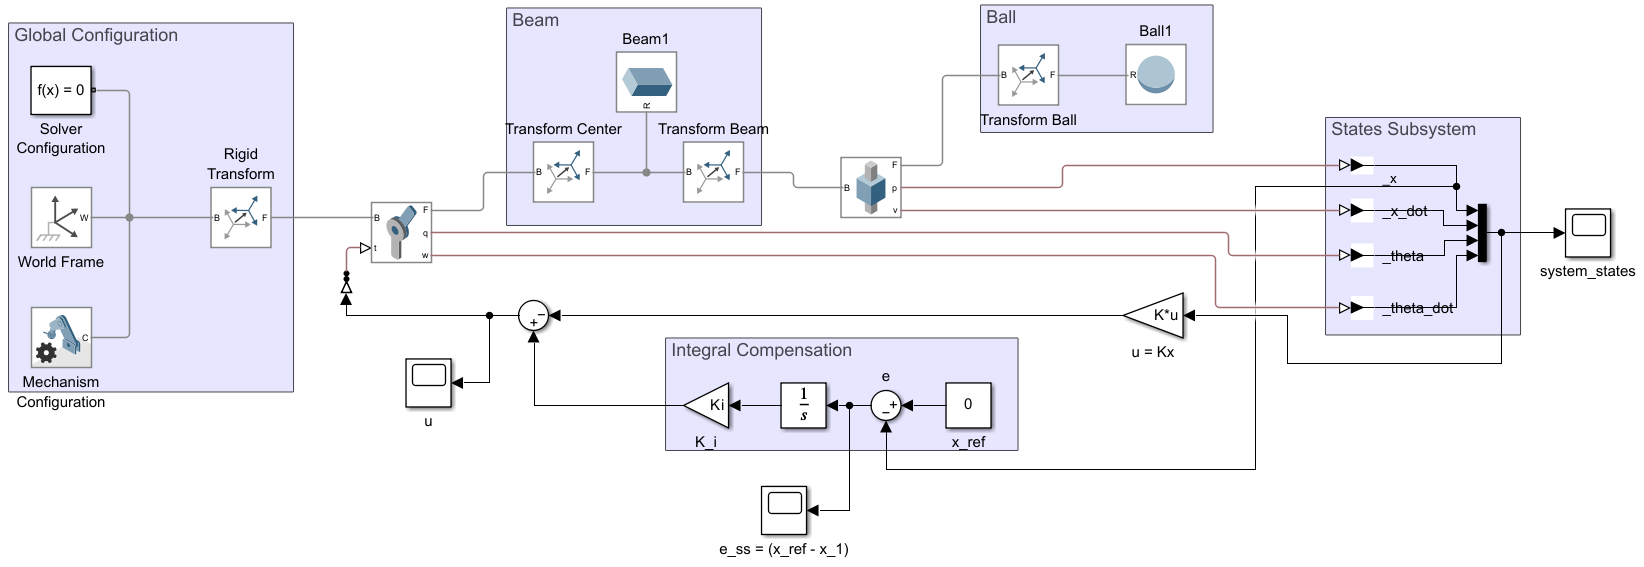
\includegraphics[width=\linewidth]{figures/simulink_model.png}
    \caption{Simulink model of the ball-and-beam system with integrated state feedback control.}
    \label{fig:simulink_model}
\end{figure}

Figures~\ref{fig:state_compare} and~\ref{fig:control_input_compare} compare state responses and control inputs, and the physical response of the system is visualized for both controllers simultaneously in Figure . The LQR controller ensures smoother trajectories and lower control effort, while the Pole Placement controller achieves faster stabilization with increased oscillations.

\begin{figure}[H]
    \centering
    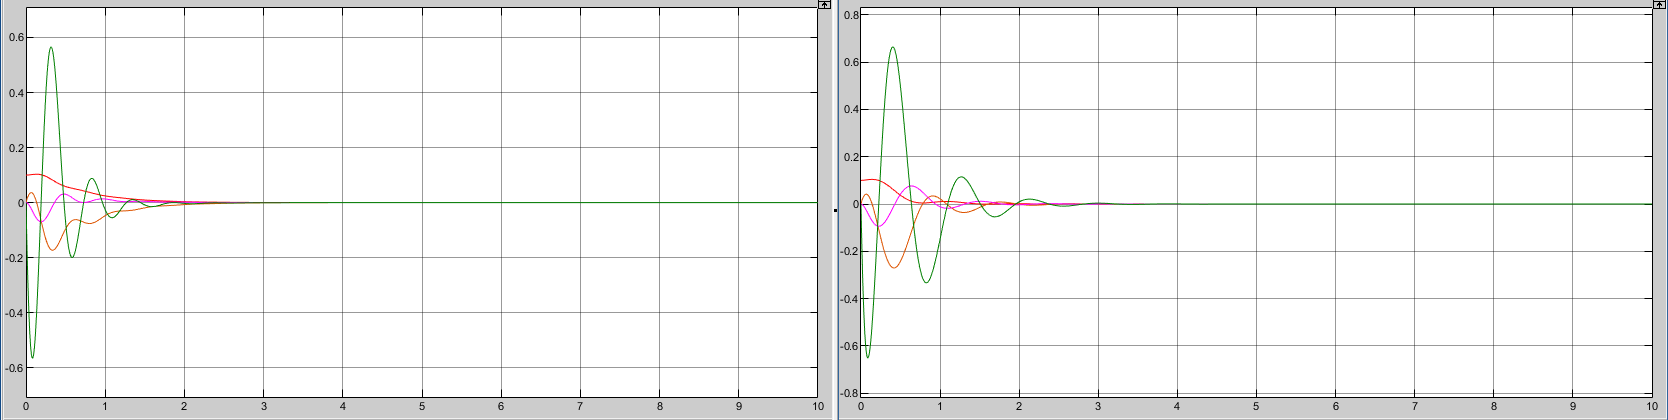
\includegraphics[width=0.6\linewidth]{figures/states_compare_scope.png}
    \caption{State Response Comparison for Pole Placement (\(K_{\text{acker}}\)) and LQR (\(K_{\text{lqr}}\)) Controllers.}
    \label{fig:state_compare}
\end{figure}

\begin{figure}[H]
    \centering
    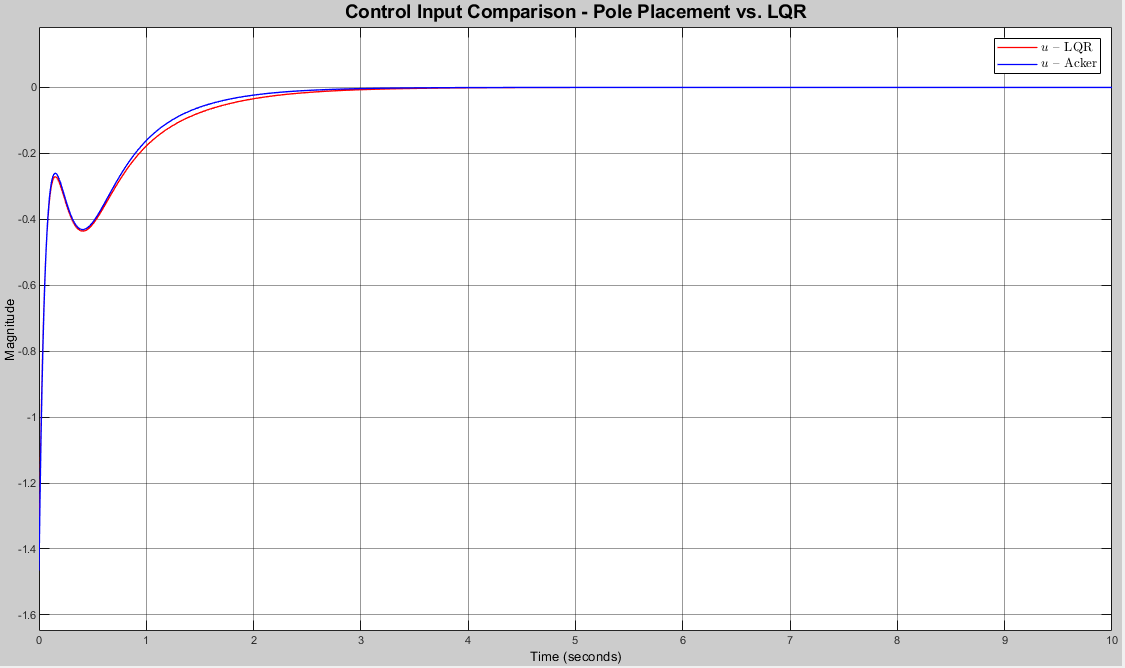
\includegraphics[width=0.6\linewidth]{figures/control_input_compare.png}
    \caption{Control Input Comparison for Pole Placement (\(K_{\text{acker}}\)) and LQR (\(K_{\text{lqr}}\)) Controllers.}
    \label{fig:control_input_compare}
\end{figure}

\subsection{Sensitivity Analysis: Effect of Mass and Beam Length Variations}
\label{subsec:sensitivity_analysis}

To analyze the robustness of the controllers, the ball's mass (\(m\)) and the beam's length (\(L\)) were varied. The mass was altered between \(m = 0.25\, \mathrm{kg}\) and \(m = 0.75\, \mathrm{kg}\), while the beam length was changed from \(L = 1.25\, \mathrm{m}\) to \(L = 1.75\, \mathrm{m}\). These variations allowed for a detailed evaluation of the system's response and control input under changing dynamics.

Figure~\ref{fig:states_varrying} illustrates the state variable responses for the two controllers under these variations. The results demonstrate that the LQR controller consistently maintains smoother responses, while the Pole Placement controller exhibits higher sensitivity to parameter changes, particularly in transient behaviors.

\begin{figure}[H]
    \centering
    \includegraphics[width=1\linewidth]{Figures/states_varrying.PNG}
    \caption{State Variable Responses Under Parameter Variations. 
    The figure illustrates the effect of varying the beam length (\(L\)) and ball mass (\(m\)) on state variable responses. 
    Top-left: \(L = 0.75\), Bottom-left: \(L = 1.25\), Top-right: \(m = 0.25\), Bottom-right: \(m = 0.75\). Responses are shown for both LQR and Pole Placement controllers.}
    \label{fig:states_varrying}
\end{figure}

The control input effort, shown in Figure~\ref{fig:input_varrying}, highlights a similar trend. The LQR controller requires smoother and less aggressive inputs, minimizing actuator stress, while the Pole Placement controller generates higher peaks and oscillations, especially for larger variations in mass and length.

\begin{figure}[H]
    \centering
    \includegraphics[width=1\linewidth]{Figures/input_varrying.PNG}
    \caption{Control Input Effort Under Parameter Variations. 
    The figure illustrates the effect of varying the beam length (\(L\)) and ball mass (\(m\)) on control input effort (\(u\)). 
    Top-left: \(L = 0.75\), Bottom-left: \(L = 1.25\), Top-right: \(m = 0.25\), Bottom-right: \(m = 0.75\). Control inputs are shown for both LQR and Pole Placement controllers.}
    \label{fig:input_varrying}
\end{figure}

These findings emphasize the robustness of the LQR controller in maintaining stability and energy efficiency across varying system parameters. In contrast, while the Pole Placement controller achieves rapid stabilization, its performance is more sensitive to parameter variations, leading to higher control effort and transient oscillations.

\begin{figure}[H]
    \centering
    \includegraphics[width=1\linewidth]{Figures/simulink_dual.PNG}
    \caption[short]{3-Dimensional visualization of controller effect on a physical model. 
    Note: Parameter values were adjusted from the specified settings to illustrate simultaneous visualization. Poles provided to the \(K_{\text{acker}}\) function were \([-50, -1+5i, -1-5i, -2.5]\).}
    \label{fig:3d_model}
\end{figure}
\section{Conclusion and Future Work}
\label{sec:conclusion}

\subsection{Conclusion}
This study presented a detailed exploration of modeling and controlling the ball-and-beam system, a paradigmatic example of instability in control theory. The system's dynamics were derived using both Newtonian and Lagrangian mechanics to provide complementary insights, and the equations were linearized to facilitate modern control design. A state-space representation was then developed, laying the groundwork for implementing advanced feedback controllers.

Two control strategies were designed and evaluated: pole placement via Ackermann’s formula and the Linear Quadratic Regulator (LQR). Both controllers effectively stabilized the ball-and-beam system, but their performance characteristics differed under varying conditions. The pole placement method achieved rapid stabilization but exhibited higher sensitivity to parameter variations, resulting in significant transient oscillations and increased control effort when system parameters, such as ball mass or beam length, were altered. In contrast, the LQR controller provided a more robust and systematic approach, excelling in minimizing oscillations, achieving smoother transient behavior, and balancing performance with energy efficiency.

The sensitivity analysis revealed that both controllers are affected by parameter variations, but the LQR controller demonstrated greater robustness. It consistently produced smoother responses and required less aggressive control inputs, minimizing actuator stress. These results highlight the importance of accounting for parameter variations in the design of controllers for systems with dynamic or uncertain operating conditions.

This work underscores the significance of rigorous system modeling and iterative refinement in control design. It also demonstrates the practical advantages of LQR controllers for stabilizing inherently unstable systems, offering valuable insights into their real-world applicability.

\subsection{Future Work}
Future research can enhance the findings of this study by focusing on the following areas:

\subsubsection{Adaptive and Robust Control}
Developing adaptive control strategies, such as gain-scheduling or self-tuning controllers, would allow dynamic adjustments to parameter variations. Robust control methods can mitigate uncertainties and disturbances.

\subsubsection{Nonlinear Control Techniques}
Exploring nonlinear control techniques, such as sliding mode control or backstepping, could address the nonlinearities inherent in the ball-and-beam system and extend performance beyond linear models.

\subsubsection{Hardware Implementation}
Applying the proposed controllers to physical systems would validate their performance under real-world conditions, addressing practical issues like noise, delays, and actuator limitations.

\subsubsection{Parameter Sensitivity Compensation}
Real-time parameter estimation methods, such as Kalman filters or adaptive observers, could enhance robustness by dynamically compensating for parameter changes.

\subsubsection{Energy Optimization}
Energy-efficient control designs can reduce actuator wear and operational costs, particularly in systems with limited resources or frequent parameter changes.

\subsubsection{Multivariable Systems}
Extending control strategies to multivariable systems, such as ball-on-sphere systems, would generalize these findings and address challenges in higher-dimensional control systems.


By addressing these areas, future work can further refine control strategies for unstable and dynamic systems, enhancing their robustness, efficiency, and real-world applicability.


\section*{Acknowledgment}
The author extends special thanks to Jonathan Shreve and Garret Smith for their innovative contributions, particularly in developing the backsolving approach that facilitated a direct comparison between the Pole Placement and LQR strategies.

\bibliographystyle{IEEEtran}
\bibliography{references}


\end{document}
